\newcommand{\figureAVRMemory}[1]{
  \def\lang{\detokenize{#1}}
  \def\langRu{\detokenize{ru}}
  \def\langEn{\detokenize{en}}
  \def\figureCaption{XXX: No translation.}
  \ifx \lang\langRu
  \def\figureCaption{
    Карта памяти AVR.
  }
  \fi
  \ifx \lang\langEn
  \def\figureCaption{
    AVR memory map.
  }
  \fi
  \begin{figure}[H]
    \centering
    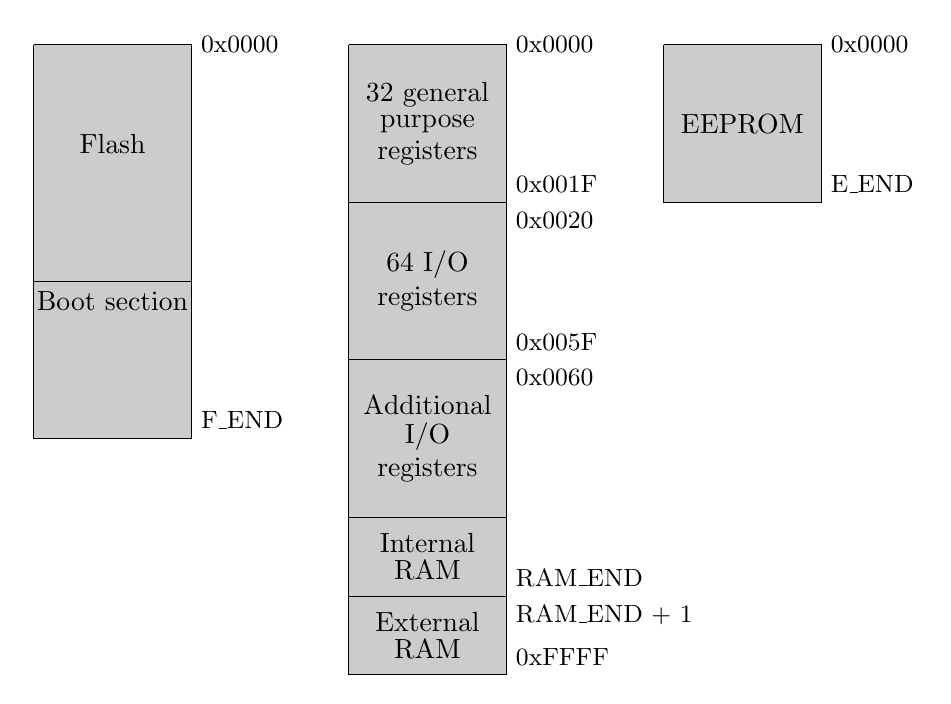
\begin{tikzpicture}
      \path[shape=coordinate]
      (0,5) coordinate(b1) (2,5) coordinate(b2)
      (2,2) coordinate(b3) (0,2) coordinate(b4);
      \filldraw[fill=white!80!black] (b1) -- (b2) -- (b3) -- (b4) -- (b1);
      \draw (1, 3.5) node[anchor=south] {Flash};
      \draw (b2) node[anchor=west] {\small{0x0000}};

      \path[shape=coordinate]
      (0,0) coordinate(b5) (2,0) coordinate(b6);
      \filldraw[fill=white!80!black] (b3) -- (b4) -- (b5) -- (b6) -- (b3);
      \draw (1, 1.5) node[anchor=south] {Boot section};
      \draw (b6) node[anchor=south west] {\small{F\_END}};

      \path[shape=coordinate]
      (4,5) coordinate(b7) (6,5) coordinate(b8)
      (6,3) coordinate(b9) (4,3) coordinate(b10);
      \filldraw[fill=white!80!black] (b7) -- (b8) -- (b9) -- (b10) -- (b7);
      \draw (5, 4) node[anchor=center] {
        \shortstack{32 general \\  purpose \\ registers}
      };
      \draw (b8) node[anchor=west] {\small{0x0000}};
      \draw (b9) node[anchor=south west] {\small{0x001F}};

      \path[shape=coordinate]
      (4,3) coordinate(b11) (6,3) coordinate(b12)
      (6,1) coordinate(b13) (4,1) coordinate(b14);
      \filldraw[fill=white!80!black] (b11) -- (b12) -- (b13) -- (b14) -- (b11);
      \draw (5, 2) node[anchor=center] {
        \shortstack{64 I/O \\ registers}
      };
      \draw (b12) node[anchor=north west] {\small{0x0020}};
      \draw (b13) node[anchor=south west] {\small{0x005F}};
      \draw (b13) node[anchor=north west] {\small{0x0060}};

      \path[shape=coordinate]
      (4,1) coordinate(b14) (6,1) coordinate(b15)
      (6,-1) coordinate(b16) (4,-1) coordinate(b17);
      \filldraw[fill=white!80!black] (b14) -- (b15) -- (b16) -- (b17) -- (b14);
      \draw (5, 0) node[anchor=center] {
        \shortstack{Additional \\ I/O \\ registers}
      };

      \path[shape=coordinate]
      (4,-1) coordinate(b18) (6,-1) coordinate(b19)
      (6,-2) coordinate(b20) (4,-2) coordinate(b21);
      \filldraw[fill=white!80!black] (b18) -- (b19) -- (b20) -- (b21) -- (b18);
      \draw (5, -1.5) node[anchor=center] {
        \shortstack{Internal \\ RAM}
      };
      \draw (b20) node[anchor=south west] {\small{RAM\_END}};
      \draw (b20) node[anchor=north west] {\small{RAM\_END + 1}};

      \path[shape=coordinate]
      (4,-2) coordinate(b22) (6,-2) coordinate(b23)
      (6,-3) coordinate(b24) (4,-3) coordinate(b25);
      \filldraw[fill=white!80!black] (b22) -- (b23) -- (b24) -- (b25) -- (b22);
      \draw (5, -2.5) node[anchor=center] {
        \shortstack{External \\ RAM}
      };
      \draw (b24) node[anchor=south west] {\small{0xFFFF}};

      \path[shape=coordinate]
      (8,5) coordinate(b26) (10,5) coordinate(b27)
      (10,3) coordinate(b28) (8,3) coordinate(b29);
      \filldraw[fill=white!80!black] (b26) -- (b27) -- (b28) -- (b29) -- (b26);
      \draw (9, 4) node[anchor=center] {
        \shortstack{EEPROM}
      };
      \draw (b27) node[anchor=west] {\small{0x0000}};
      \draw (b28) node[anchor=south west] {\small{E\_END}};
    \end{tikzpicture}
    \caption{\figureCaption}
    \label{fig:avr-memory}
  \end{figure}
}
